\section{Objetivos}
\begin{itemize}
    \item Identificar la presencia de cargas eléctricas en diferentes tipos de objetos materiales, explorando cómo se manifiestan las cargas en el entorno cotidiano.
    \item Reconocer dos tipos de interacciones eléctricas y dos tipos de cargas eléctricas, diferenciando entre cargas positivas y negativas y su influencia mutua.
    \item Medir el campo eléctrico de una esfera cargada a diferentes distancias, utilizando instrumentos de medición para cuantificar las variaciones del campo eléctrico y su dependencia con la distancia.
\end{itemize}

\section{Marco Teórico}
La teoría que fundamenta este laboratorio se basa en el concepto de \textbf{electrostática}, que estudia las cargas eléctricas en reposo. Cuando dos cuerpos diferentes se frotan, ocurre un intercambio de electrones, llevando a que uno de los cuerpos gane electrones y se cargue negativamente, mientras que el otro los pierde y se carga positivamente. Este fenómeno es evidente en ejemplos cotidianos como el frotamiento de vidrio con seda o ámbar con piel.
\newline \hfill \break
La \textbf{Ley de Coulomb} es central en este contexto, estableciendo que la fuerza entre dos cargas es directamente proporcional al producto de las cargas e inversamente proporcional al cuadrado de la distancia entre ellas. Esta ley se expresa matemáticamente como:
\[
\vec{F} = k \frac{Q_1 \cdot Q_2}{r^2} \hat{r}
\]
donde:
\begin{itemize}
    \item $ \vec{F} $ es la fuerza entre las cargas.
    \item $ Q_1 $ y $ Q_2 $ son las magnitudes de las dos cargas.
    \item $ r $ es la distancia entre las cargas.
    \item $ k $ es la constante de Coulomb, $9 \times 10^9 \text{ Nm}^2/\text{C}^2$.
\end{itemize}

El \textbf{campo eléctrico} ($ \vec{E} $), definido como la fuerza por unidad de carga, proporciona un medio para describir la interacción eléctrica en un punto del espacio debido a la presencia de otras cargas. Si una carga de prueba $ q $ se coloca en un campo eléctrico, la fuerza que experimenta es:
\[
\vec{F} = q \cdot \vec{E}
\]

Este campo es crucial para entender cómo las cargas influyen en su entorno y es calculado para diferentes configuraciones de carga en el laboratorio, usando instrumentos específicos como el medidor de campo eléctrico.

\section{Análisis y discusión: Montaje 1}

\subsection{Interacción entre barras y papel}
\textbf{Recorte pequeños trocitos de papel y reúnalos; luego tome la barra de vidrio y frótela con
seda; acérquela a los trocitos de papel. Repita este proceso con una barra de plástico
frotándola con piel. Describa lo que ocurre.} Los papelitos se ven atraídos por ambos materiales, pero en el caso de la barra de plástico, se observa que hay más cantidad atraída.

\subsubsection{Causa de la atracción}
\textbf{Explique por qué los trocitos de papel son atraídos por la barra de plástico y también por la barra de vidrio.} Al frotar las barras con seda y piel, respectivamente, la barra de vidrio adquiere carga positiva y la barra de plástico carga negativa. Esta diferencia de cargas genera una fuerza electrostática que atrae a los trozos de papel, los cuales son ligeros y pueden ser fácilmente influenciados por estas fuerzas.

\subsection{Interacción entre barras de vidrio y plástico}
\textbf{Frote una barra de vidrio con un pedazo de seda y colóquela en una base giratoria; procure
que la barra se quede quieta. Luego frote otra barra de plástico con piel y acérquela a la
barra de vidrio anterior, en el extremo que hizo el frotamiento. Describa lo que ocurre.} La barra de vidrio, cargada positivamente, se ve atraída por la barra de plástico, cargada negativamente, causando que la barra de vidrio en la base giratoria empiece a rotar hacia la barra de plástico.

\subsection{Interacción entre dos barras de plástico}
\textbf{Repita el numeral anterior con dos barras de plástico frotadas con piel. Describa lo que
ocurre.} Al ser ambas barras de plástico cargadas negativamente por la fricción con la piel, se repelen entre sí, lo que causa que la barra en la base giratoria se mueva en sentido contrario, demostrando la repulsión entre cargas iguales.

\subsection{Identificación y Verificación de Cargas}
\textbf{Explique o describa un diseño experimental sencillo que permita:}
\subsubsection{Diseño Experimental para Identificación de Cargas}
\textbf{Identificar la existencia de carga eléctrica en un material.} Utilizar un electroscopio. Al acercar un material previamente frotado a la esfera del electroscopio, las hojas de metal dentro del dispositivo se separarán si el material está cargado, debido a la repulsión entre cargas del mismo tipo.

\subsubsection{Diseño Experimental para Verificación de Tipos de Cargas}
\textbf{Verificar la existencia de dos tipos de carga eléctrica.} Se puede utilizar un kit de electrización por contacto y fricción. Frotar diferentes materiales y acercarlos a un electroscopio cargado negativamente. Si las hojas se separan más, el objeto está cargado negativamente; si se juntan, está cargado positivamente.

\subsection{Cargando Esferas Metálicas}
\textbf{Indique cómo se pueden cargar dos esferas metálicas aisladas del mismo material y
tamaño. Haga una secuencia de gráficos que relacione la situación correspondiente:}
\subsubsection{Esferas con Cargas de Signos Opuestos}
\textbf{Cargar dos esferas metálicas aisladas con cargas de igual magnitud pero signos diferentes.} Utilizar un generador Van de Graaff. Colocar una esfera en contacto con el generador para cargarla positivamente y la otra esfera en contacto con la tierra para cargarla negativamente, y luego aislar ambas.

\subsubsection{Esferas con Cargas del Mismo Signo}
\textbf{Cargar dos esferas metálicas aisladas con cargas de igual magnitud e igual signo.} Utilizar dos generadores Van de Graaff, uno configurado para cargar positivamente y otro para cargar negativamente, y cargar ambas esferas con el mismo tipo de carga.

\subsection{Experimentación con Conexión a Tierra}
\textbf{Considere la siguiente situación: Se aproxima una carga negativa a un conductor aislado sin
carga, el conductor se aterriza (se conecta a tierra) mientras la carga está cerca.}
\subsubsection{Efecto de la Conexión a Tierra}
\textbf{¿El conductor se carga cuando se acerca una carga negativa y se conecta a tierra?} Sí. Los electrones en el conductor se mueven hacia la tierra dejando un déficit de electrones (carga positiva) debido a la repulsión con la carga negativa cercana.

\subsubsection{Retiro de Carga y Conexión a Tierra}
\textbf{¿Se carga el conductor si se retira la carga y luego la conexión a tierra?} No. Una vez que el conductor ha sido conectado a tierra y luego desconectado, cualquier exceso de carga ya ha sido neutralizado; por lo tanto, no retiene carga adicional.

\subsubsection{Supresión de la Conexión a Tierra y Retiro de Carga Externa}
\textbf{¿Se carga el conductor si se suprime la conexión a tierra y luego se retira la carga externa?} No. Sin la conexión a tierra, el conductor no puede disipar el exceso de carga durante la presencia de la carga externa, y una vez retirada la carga externa, no hay un mecanismo que induzca una carga en el conductor.

\subsection{Verificación del Comportamiento de Conductores y No Conductores}
\textbf{¿Cómo verificar el comportamiento de materiales conductores y no conductores?} Se puede demostrar utilizando un electroscopio. Conectando diferentes materiales al electroscopio y observando la respuesta de las hojas metálicas, se puede determinar si el material permite el flujo de electrones (conductor) o no (aislante).

\subsection{Carga en Vidrio y Ámbar}
\textbf{¿Por qué el vidrio se carga positivamente y el ámbar negativamente?} Esto se debe a la tendencia de estos materiales a perder o ganar electrones, respectivamente. El vidrio tiende a perder electrones cuando se frota con seda, adquiriendo una carga positiva, mientras que el ámbar tiende a ganar electrones cuando se frota con piel, adquiriendo una carga negativa.

\section{Procedimiento Experimental y Resultados: Montaje 2}

\subsection{Leer medidas con el generador de Van de Graaff}
\textbf{Con el generador Van der Graaff, cargar una esfera conductora previamente colocada
sobre una base aislante. Con el medidor de campo eléctrico, tomar y reportar las medidas
del voltaje generado por la bola conductora a las distancias mostradas en la siguiente
tabla:}
\begin{figure}[H]
    \centering
    \begin{subfigure}[b]{\textwidth}
        \centering
        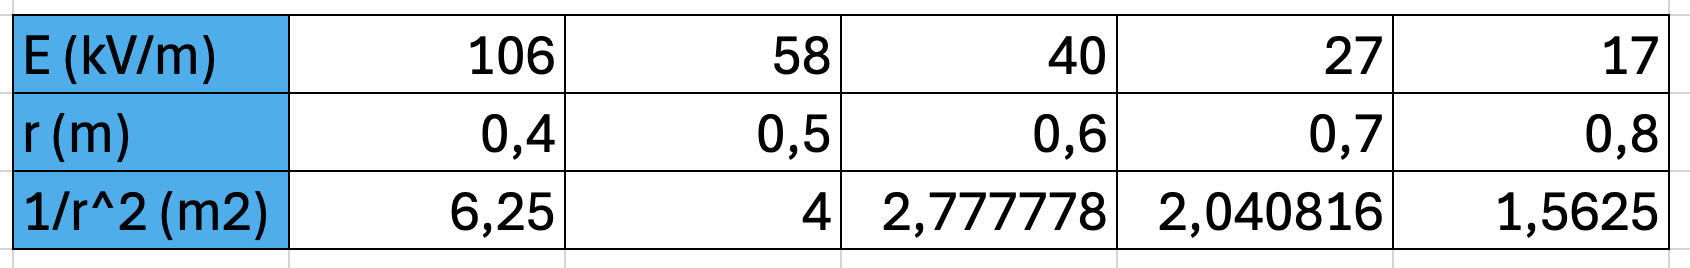
\includegraphics[width=\textwidth]{Figures/1. Content/tablaCampoVSR2.png}
        \caption{Tabla Campo eléctrico $E$, $r$ y $r^{-2}$}
        \label{fig: tabla Campo vs r^-2}
    \end{subfigure}
    \hfill
\end{figure}

\subsection{De la gráfica campo eléctrico $E$ vs $r^{-2}$:}

\begin{figure}[H]
    \centering
    \begin{subfigure}[b]{\textwidth}
        \centering
        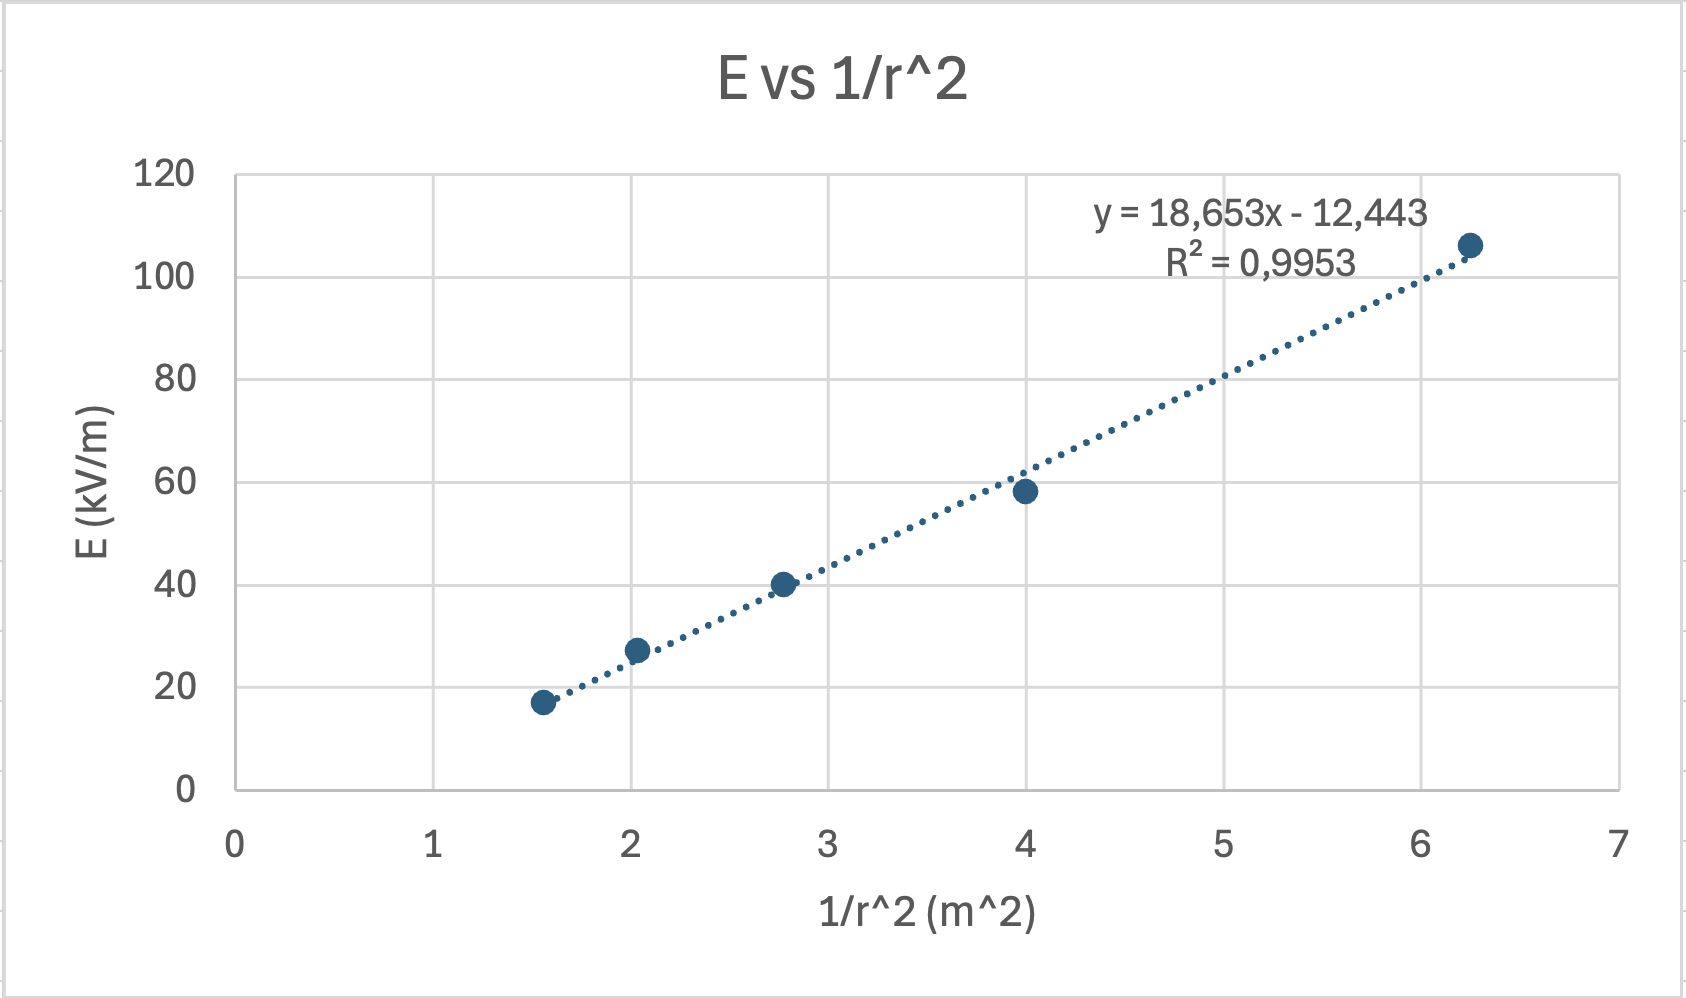
\includegraphics[width=0.8\textwidth]{Figures/1. Content/campoVSR2.png}
        \caption{Campo eléctrico $E$ vs $r^{-2}$}
        \label{fig: Campo vs r^-2}
    \end{subfigure}
    \hfill
\end{figure}

\subsubsection{¿Cuál es la ecuación del gráfico?}

La ecuación de la recta ajustada a los datos, según la gráfica, es:
\[
E = 18.653 \cdot \left(\frac{1}{r^2}\right) - 12.443
\]
donde:
\begin{itemize}
    \item \( E \) es el campo eléctrico en kV/m.
    \item \( \frac{1}{r^2} \) es el inverso del cuadrado de la distancia en m\(^2\).
\end{itemize}

\subsubsection{¿Qué significado físico tienen la pendiente y el intercepto de la recta de ajuste
por mínimos cuadrados?}
\begin{itemize}
    \item \textbf{Pendiente (18.653 kV·m\(^2\)):} La pendiente de la recta en una gráfica de \( E \) versus \( \frac{1}{r^2} \) está relacionada con la constante de proporcionalidad en la ley de Coulomb, es decir, \( k \cdot Q \), donde \( k \) es la constante de Coulomb y \( Q \) es la carga de la fuente. En este caso, la pendiente nos da una medida de \( k \cdot Q \), ajustada a las unidades del sistema de medición.
    \item \textbf{Intercepto (-12.443 kV/m):} El intercepto idealmente debería ser cero según la ley teórica de Coulomb, ya que \( E \) debería ser cero cuando \( r \) tiende a infinito (\(\frac{1}{r^2} = 0\)). Un intercepto negativo puede indicar una desviación en la calibración del instrumento o la presencia de un campo eléctrico de fondo.
\end{itemize}

\subsubsection{¿Qué unidades tienen la pendiente y el intercepto de la recta de ajuste?}
\begin{itemize}
    \item \textbf{Unidades de la Pendiente:} Las unidades de la pendiente son kV·m\(^2\), lo cual es consistente con la forma de la ecuación \( E = k \frac{Q}{r^2} \), donde \( E \) está en kV/m y \( \frac{1}{r^2} \) en m\(^{-2}\).
    \item \textbf{Unidades del Intercepto:} Las unidades del intercepto son kV/m, que son las mismas unidades que las del campo eléctrico \( E \).
\end{itemize}

\section{Causas de Error}
Las principales causas de error en este experimento podrían incluir:
\begin{itemize}
    \item Errores en la calibración del medidor de campo eléctrico que podrían haber afectado la precisión de las mediciones.
    \item Influencias externas como campos electromagnéticos no controlados en el laboratorio que podrían haber interferido con las mediciones.
    \item Inexactitudes en la medición de distancias que podrían haber introducido variaciones en los resultados.
    \item No alinear perfectamente el sensor con el centro de la esfera cargada, lo que podría alterar los valores medidos.
    \item La pérdida de carga de la esfera durante el experimento debido a condiciones ambientales como la humedad o aislamiento inadecuado.
\end{itemize}

\section{Conclusiones}
A partir del experimento realizado, se pueden extraer las siguientes conclusiones:
\begin{itemize}
    \item El experimento demostró efectivamente la presencia de cargas eléctricas en diferentes materiales y cómo estas se manifiestan al interactuar con su entorno.
    \item Se observaron y confirmaron dos tipos fundamentales de interacciones eléctricas: la atracción entre cargas opuestas y la repulsión entre cargas iguales.
    \item Las mediciones del campo eléctrico corroboraron la relación inversamente proporcional entre el campo eléctrico y el cuadrado de la distancia a la fuente de carga, proporcionando una validación empírica robusta de la Ley de Coulomb.
    \item Los resultados experimentales, alineados estrechamente con los principios teóricos, refuerzan la comprensión de las leyes fundamentales de la electrostática y su aplicabilidad en contextos reales.
\end{itemize}